\chapter{Methodology}
\label{chap:methodology}

\section{Objectives}

The main objective of this experiment is to assess whether RSSI values from ESP32 BLE beacons can reliably determine a smartphone’s position and detect user proximity to a predefined location within a threshold of three meters or less. This validation is crucial for ensuring that the proposed indoor localization system can accurately detect a user's presence near a point of interest (POI).

In addition to the primary objective, secondary goals include evaluating the impact of environmental factors on localization accuracy and analyzing the system’s responsiveness when the user moves dynamically. Finally, the experiment will compare localization accuracy across different smartphone models to determine whether variations in hardware affect the system’s performance.

\section{Experimental Setup}

\subsection{Hardware and System Architecture}

The experimental setup comprises up to four ESP32 devices running a custom firmware that enables them to operate as BLE beacons. These devices periodically broadcast BLE signals. When network access is available, they upload their position to an MQTT broker; otherwise, they function solely as standalone BLE beacons.

A smartphone application is responsible for collecting and processing the beacon signals. This application retrieves a list of authorized BLE beacon signatures from the MQTT broker and continuously scans for nearby devices that match these known signatures. No user data is transmitted from the smartphone to the server, ensuring privacy for both the user and other individuals within the area.

\subsection{Application Features and Localization Logic}

The smartphone application provides a real-time graphical interface that visualizes the localization process, primarily for debugging and in-depth analysis. A map displays the static positions of the beacons, with each beacon represented by a circle corresponding to the estimated distance from the phone. Additionally, a dot indicates the estimated position of the smartphone, while crosses mark are the predefined points of interest.

Localization is based on RSSI-based triangulation. A phone is considered to be within a POI when it has been detected at least twice within a three-meter radius. Conversely, the phone is considered to have exited the POI if it is subsequently detected twice at a location beyond five meters. This difference between the entry and exit thresholds is implemented to prevent unstable state changes between being inside and outside a POI. These threshold values have been determined based on preliminary evaluations and may be adjusted for different experimental conditions, depending on beacon placement, artwork density, and the complexity of the indoor environment.

\section{Experimental Procedure}

To systematically evaluate the performance of the system, and it's value within a museum, four distinct experiments will be conducted. These experiments focus on evaluating localization accuracy, differences in smartphone models, impact of museum layouts and its operations within a museum.

\subsection{Experimental layout}

The first experiment will take place in a designated corridor within the university, while the others are directly on a floor of the museum. ESP32 beacons will  be installed at predefined locations to provide adequate coverage of all POIs. The POIs correspond to specific reference points where localization should occur accurately. Participants performing the tests will execute a predefined sequence of movements, ensuring uniformity in data collection and minimizing variability caused by human movement patterns.

Localization data, including timestamps for detected entries, exits, and continuous tracking points, will be logged during all experiments. Additionally, manual records will be kept to compare the system's performance with a ground truth reference, ensuring accurate evaluation.

\subsection{Experiment 1: Localization Accuracy}
\label{exp:1_accuracy}

The first experiment focus on the beacons data directly. It aims to calibrate the meta-parameters and analyzes the precision of the distance estimation between the phone and the beacons. The experiment take place in a corridor, with no obstacle and a direct Line of Sight (LoS) between the phone and the sensors. The sensor is placed at 1.5 meters from the ground and measurements are taken at every meter, starting at "0" ($L_0$), with the phone touching the sensor, and up to 15 meters away from it ($L_{15}$). At each step, the phone take measurements for 20 seconds. Each sensor is tested with no other sensor active at the same time to minimize inteferences.

\begin{figure}[H]
    \centering
    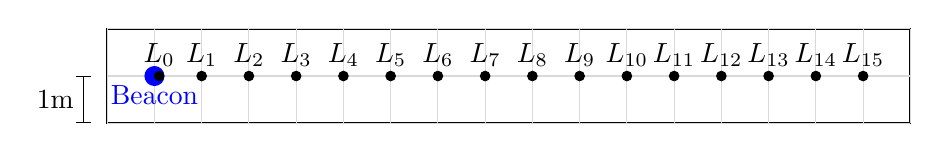
\begin{tikzpicture}[scale=0.6]
        % Room dimensions 
        \draw[thick] (0,0) rectangle (17,2);  
        % Grid (optional, for reference)
        \draw[gray!30, step=1] (0,0) grid (17, 2);
        
        % ESP32 devices (blue dots)
        \filldraw[blue] (1, 1) circle (0.2) node[below] {Beacon};

        % User positions (X marks)
        \filldraw (1.1, 1) circle (0.1) node[above] {$L_0$};
        \filldraw (2, 1) circle (0.1) node[above] {$L_1$};
        \filldraw (3, 1) circle (0.1) node[above] {$L_2$};
        \filldraw (4, 1) circle (0.1) node[above] {$L_3$};
        \filldraw (5, 1) circle (0.1) node[above] {$L_4$};
        \filldraw (6, 1) circle (0.1) node[above] {$L_5$};
        \filldraw (7, 1) circle (0.1) node[above] {$L_6$};
        \filldraw (8, 1) circle (0.1) node[above] {$L_7$};
        \filldraw (9, 1) circle (0.1) node[above] {$L_8$};
        \filldraw (10, 1) circle (0.1) node[above] {$L_9$};
        \filldraw (11, 1) circle (0.1) node[above] {$L_{10}$};
        \filldraw (12, 1) circle (0.1) node[above] {$L_{11}$};
        \filldraw (13, 1) circle (0.1) node[above] {$L_{12}$};
        \filldraw (14, 1) circle (0.1) node[above] {$L_{13}$};
        \filldraw (15, 1) circle (0.1) node[above] {$L_{14}$};
        \filldraw (16, 1) circle (0.1) node[above] {$L_{15}$};
        
        % Scale indicator
        \draw[|-|] (-0.5,0) -- (-0.5,1) node[midway, left] {1m};
    \end{tikzpicture}
    \caption{Experimental setup for the first experiment showing one beacon and all the references distances.}
    \label{fig:exp1_setup}
\end{figure}

\subsection{Experiment 2: Impact of museum layout}
\label{exp:2_museum}

The second experiment focus on the impact of the museum layout on the results. It takes places directly inside the museum on the floor used for this experimentation. All the devices are on the floor, and the user keep the smartphone in hand, in front of him. The user follow the path across the 8 locations, following the order $L_0 \rightarrow L_1 \rightarrow~...~\rightarrow L_8$. Only the data at the different locations are considered, so the path between them has no impact on the results. Points $L_{0,1,2,4,5,8}$ are inside the covered area while $L_{3,6,7}$ are outside of it, in order to analyze the behavior in this edge case. The direct Lines of Sight (LoS) are never guaranteed between the beacons and the phone.

\begin{figure}[H]
    \centering
    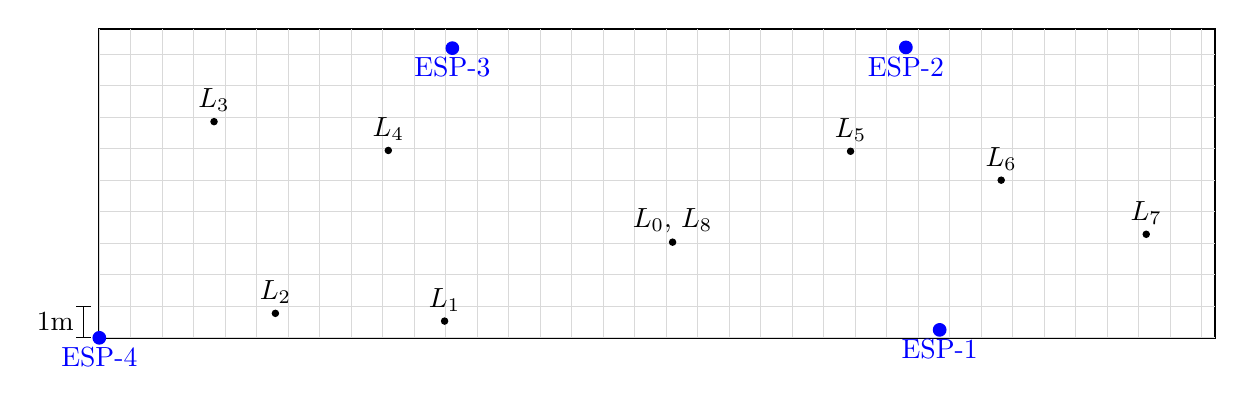
\begin{tikzpicture}[scale=0.4]
        % Room dimensions 
        \draw[thick] (0,0) rectangle (35.417, 9.812);  
        % Grid (optional, for reference)
        \draw[gray!30, step=1] (0,0) grid (35.417, 9.812);
        
        % ESP32 devices (blue dots)
        \filldraw[blue] (26.681, 0.252) circle (0.2) node[below] {ESP-1};
        \filldraw[blue] (25.608, 9.221) circle (0.2) node[below] {ESP-2};
        \filldraw[blue] (11.209, 9.197) circle (0.2) node[below] {ESP-3};
        \filldraw[blue] (0, 0) circle (0.2) node[below] {ESP-4};

        % User positions (X marks)
        \filldraw (18.201, 3.037) circle (0.1) node[above] {$L_0$, $L_8$};
        \filldraw (10.962, 0.531) circle (0.1) node[above] {$L_1$};
        \filldraw (5.590, 0.777) circle (0.1) node[above] {$L_2$};
        \filldraw (3.642, 6.864) circle (0.1) node[above] {$L_3$};
        \filldraw (9.175, 5.949) circle (0.1) node[above] {$L_4$};
        \filldraw (23.852, 5.923) circle (0.1) node[above] {$L_5$};
        \filldraw (28.635, 5.005) circle (0.1) node[above] {$L_6$};
        \filldraw (33.240, 3.287) circle (0.1) node[above] {$L_7$};
        
        % Scale indicator
        \draw[|-|] (-0.5,0) -- (-0.5,1) node[midway, left] {1m};
    \end{tikzpicture}
    \caption{Experimental setup for the second experiment showing the beacons and some reference points.}
    \label{fig:exp2_museum}
\end{figure}

\subsection{Experiment 3: Detecting POI and providing meaningful data}
% Seek for supervisor's opinions

The third experiment focus on the user experience within the exhibition. It has been chosen here to provide to the user two layers of information trough it's visit. First, an overview by section, to provide general information about the sections and their main art pieces, then the application provide the list of the art pieces of the section and close to the visitor, and he has to ability to chose to get more information on them by interacting with the application. This way, the visitor can follow the whole floor without having to interact with the application, but only by moving around areas, but can chose to move by it's own or to get more information on the sections he wants to.

The user follow the path across the 8 locations, following the order $L_0 \rightarrow L_1 \rightarrow~...~\rightarrow L_8$. The user stay still for 20 seconds in each location, then move at a walk pace to the next one. The exact path is shown by dashed lines on the \autoref{fig:exp3_poi}. The exact time the visitor is detected in each area is recorded alongside the classical data.

\begin{figure}[H]
    \centering
    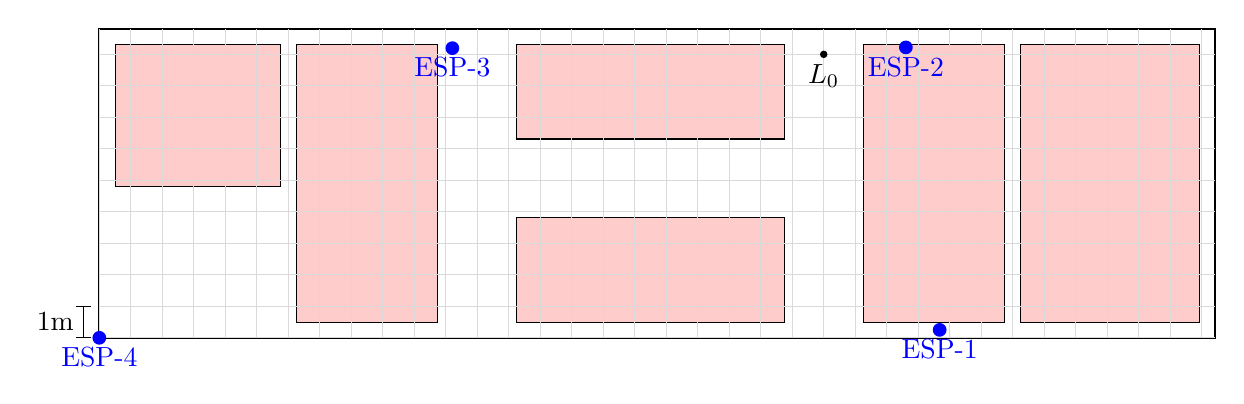
\begin{tikzpicture}[scale=0.4]
        % Room dimensions 
        \draw[thick] (0,0) rectangle (35.417, 9.812);  
        
        % Sections
        \draw[fill=red!20] (29.25, 0.5) rectangle (34.917, 9.312);
        \draw[fill=red!20] (24.25, 0.5) rectangle (28.75, 9.312);
        \draw[fill=red!20] (13.25, 6.312) rectangle (21.75, 9.312);
        \draw[fill=red!20] (13.25, 0.5) rectangle (21.75, 3.812);
        \draw[fill=red!20] (6.25, 0.5) rectangle (10.75, 9.312);
        \draw[fill=red!20] (0.5, 4.812) rectangle (5.75, 9.312);
        
        % Grid (optional, for reference)
        \draw[gray!30, step=1] (0,0) grid (35.417, 9.812);
        
        % ESP32 devices (blue dots)
        \filldraw[blue] (26.681, 0.252) circle (0.2) node[below] {ESP-1};
        \filldraw[blue] (25.608, 9.221) circle (0.2) node[below] {ESP-2};
        \filldraw[blue] (11.209, 9.197) circle (0.2) node[below] {ESP-3};
        \filldraw[blue] (0, 0) circle (0.2) node[below] {ESP-4};

        % User positions
        \filldraw (23, 9) circle (0.1) node[below] {$L_0$};
        
        % Scale indicator
        \draw[|-|] (-0.5,0) -- (-0.5,1) node[midway, left] {1m};
    \end{tikzpicture}
    \caption{Experimental setup for the third experiment showing The beacons and the POI areas.}
    \label{fig:exp3_poi}
\end{figure}

\subsection{Experiment 4: Repeat with other phones}

The fourth and last experiment aim to ensure the precision of the system with multiple other phones. 